\documentclass[conference]{IEEEtran}
\IEEEoverridecommandlockouts
% Make each author block wide enough that 3 fit on one row
\makeatletter
\def\@IEEEauthorblockconfadjspace{-0.25em}
\makeatother

\usepackage{cite}
\usepackage{amsmath,amssymb,amsfonts}
\usepackage{algorithmic}
\usepackage{graphicx}
\usepackage{textcomp}
\usepackage{xcolor}
\usepackage{booktabs}
\usepackage{hyperref}
\usepackage{enumitem}
\usepackage{multirow}

\def\BibTeX{{\rm B\kern-.05em{\sc i\kern-.025em b}\kern-.08em
    T\kern-.1667em\lower.7ex\hbox{E}\kern-.125emX}}

\begin{document}

\title{Blink: An Explainable, Topology-Aware Framework for GPU Performance Prediction in Deep Learning}

\author{
\IEEEauthorblockN{Aniket Mishra}
\IEEEauthorblockA{\textit{Dept. of Computing Technology}\\
\textit{SRM Inst. of Science and Technology}\\
Chennai, India\\
am4198@srmist.edu.in}
\and
\IEEEauthorblockN{Shivam Upadhyay}
\IEEEauthorblockA{\textit{Dept. of Computing Technology}\\
\textit{SRM Inst. of Science and Technology}\\
Chennai, India\\
su9333@srmist.edu.in}
\and
\IEEEauthorblockN{Dr. Lubin Balasubramanian}
\IEEEauthorblockA{\textit{Dept. of Computing Technology}\\
\textit{SRM Inst. of Science and Technology}\\
Chennai, India\\
lubinb@srmist.edu.in}
}

\maketitle

\begin{abstract}
Before a deep learning model ever touches production, it must survive a gauntlet of
hardware constraints: will it fit in GPU memory, and will it respond fast enough to
satisfy a service-level agreement? Today, the only reliable way to answer these
questions is to run the model and measure---a process that burns real GPU-hours during
development and becomes completely intractable inside Neural Architecture Search loops.
This paper introduces \textbf{Blink}, a framework designed to answer both questions
without executing the model at all. We extract two complementary representations from
a PyTorch \texttt{nn.Module}: a 21-dimensional static feature vector covering
parameters, FLOPs, and layer composition, and a 64-dimensional graph embedding
produced by a Graph Convolutional Network applied to the model's computational graph.
An XGBoost regressor trained on their concatenation predicts forward-pass latency and
peak VRAM consumption. What separates Blink from prior work is the addition of
SHAP-driven per-prediction attribution---and dynamically calibrated 80\% confidence
intervals generated by a unified three-quantile setup ($\tau \in \{0.1, 0.5, 0.9\}$)
rigorously evaluated via Interval Pinball Loss. Across 953 profiling measurements
spanning 57 architectures on an NVIDIA RTX~3060, Blink achieves 35.15\% MAPE on
latency and 7.84\% on memory under a random 80/20 train-test split, providing a 
genuine, robust baseline across highly diverse computational graphs.
\end{abstract}

\begin{IEEEkeywords}
Performance Prediction, Machine Learning Systems, Neural Architecture Search,
Graph Neural Networks, Explainable AI, XGBoost
\end{IEEEkeywords}

%------------------------------------------------------------------------
\section{Introduction}
%------------------------------------------------------------------------

Somewhere between a researcher writing a training script and a model actually
serving requests in production, there is a painful gap: nobody knows in advance
how much GPU memory the model needs or how long each forward pass will take.
The gap matters for several reasons. Cloud GPU instances bill by the wall-clock
second~\cite{ignatov2018ai}, so exploratory profiling has a direct dollar cost.
In shared cluster environments, jobs that over-request memory queue behind jobs
that fit; jobs that under-request get killed. And in latency-sensitive systems---
autonomous perception, video analytics, real-time recommendation---missing a timing
budget is not just inefficient, it is a correctness failure.

The conventional response is brute-force empiricism: allocate some memory, submit
a job, watch for out-of-memory errors, adjust the batch size, repeat. For a single
model this is tolerable. For Neural Architecture Search (NAS)~\cite{elsken2019neural},
where the search procedure may evaluate tens of thousands of candidate architectures,
this loop is the primary computational bottleneck. Back-of-envelope estimates put
the profiling cost of a full NAS run at months of GPU-hours~\cite{li2021hw},
most of it spent measuring latency for architectures that will never be trained.

\subsection{The Limits of Analytical Estimators}

The textbook response to expensive profiling is to replace it with a cheap proxy.
FLOPs is the most common choice: it is easy to compute, differentiable, and
intuitively connected to runtime~\cite{justus2018predicting}. The problem is that
modern GPU execution is rarely compute-bound. Memory bandwidth is the bottleneck
for a surprising fraction of common layers, and two architectures with identical
FLOP counts can differ by a factor of two or more in wall-clock time depending on
how their operations interact with the memory hierarchy. Depthwise separable
convolutions are a good illustration: they are designed to reduce FLOPs, but their
fragmented access pattern causes high kernel launch overhead and poor cache
utilisation on massively parallel hardware, so the latency saving is much smaller
than the FLOP reduction implies. Similar problems arise with parameter counts---
a 25M-parameter convolutional network and a 25M-parameter Transformer execute very
differently, yet look identical under any scalar proxy.

Data-driven approaches that regress directly on handcrafted feature
vectors~\cite{lee2021hardware} recover some of this lost signal, but they
discard graph structure entirely. A DenseNet and a VGG with similar parameter
distributions look nearly identical to a flat feature vector, even though their
memory access patterns and kernel launch sequences are fundamentally different.

\subsection{Explainability as a First-Class Requirement}

Graph Neural Networks~\cite{dudziak2020brp} address the topology gap and tend to
produce accurate latency estimates. But accuracy alone is not enough when the
predictor is embedded in a design loop. When Blink flags a candidate architecture
as too slow, the useful response is not just ``reject''---it is ``here is which
part of the design is causing the problem, and here is roughly how much.'' A pure
GNN predictor cannot provide this. Its output is a scalar; the internal reasoning
that produced it is not accessible to the user.

\subsection{Our Approach}

Blink resolves both issues through a single architectural decision: rather than
training an end-to-end deep predictor, we use the GNN purely as a feature
extractor and hand its output to XGBoost for the final regression step. Tree
ensembles support exact SHAP computation natively, so every prediction arrives
with a per-feature attribution breakdown at negligible additional cost. The
contributions of this paper are:

\begin{enumerate}
    \item \textbf{Dual-Representation Pipeline:} A feature extraction stage that
    runs static FX-tracing metrics and GCN graph encoding in parallel, capturing
    both coarse-grained architectural statistics and fine-grained topological
    structure.
    \item \textbf{Hybrid Prediction Model:} An Optuna-tuned XGBoost regressor
    that ingests the concatenated representation; the choice of tree ensembles
    over neural regression is deliberate and enables the explainability
    component.
    \item \textbf{Per-Prediction Attribution:} SHAP waterfall plots surfaced
    after every inference call, decomposing the predicted latency into
    contributions from static features and an aggregated graph topology term.
    \item \textbf{Calibrated Prediction Intervals:} A unified quantile regression
    framework extracting central medians ($\tau=0.50$) alongside bounding
    $\tau=0.10$ and $\tau=0.90$ intervals, thoroughly evaluated via Interval
    Pinball Loss and empirically validated at 80.3\% coverage.
\end{enumerate}

%------------------------------------------------------------------------
\section{Related Work}
%------------------------------------------------------------------------

\subsection{FLOPs and Analytical Bounds}

Counting multiply-accumulate operations has been the dominant cost proxy in NAS
since early reinforcement learning approaches~\cite{zoph2016neural} because the
metric is cheap and differentiable. The fundamental limitation was made concrete
by Ma et al.~\cite{ma2018shufflenet}, who showed empirically that equal-MAC
networks can differ by up to $4\times$ in measured speed when moving between GPU
microarchitectures (e.g., Turing to Ampere), a discrepancy traceable to
differences in memory bandwidth rather than compute throughput. Roofline
analysis~\cite{williams2009roofline} provides a more rigorous way to characterise
whether a kernel is compute-limited or bandwidth-limited, but applying it reliably
to the sequence of fused operations in a real PyTorch graph is difficult in
practice due to compounding approximation errors~\cite{dong2021ppp}.

\subsection{Learned Latency Predictors}

The availability of NAS-Bench-201~\cite{dong2020nas}, which tabulated measured
latencies for 15,625 discrete cell architectures, created a foundation for
learning-based prediction. BRP-NAS~\cite{dudziak2020brp} was among the earliest
systems to use GCNs for encoding operation-level graph structure, framing accuracy
and latency prediction as a joint learning problem. HELP~\cite{lee2021hardware}
approached hardware portability through meta-learning, training a predictor that
can transfer across CPU, GPU, TPU, and ASIC targets with limited additional
profiling. Both systems demonstrate that graph structure carries useful predictive
signal, but neither quantifies prediction uncertainty nor surfaces explanations.

\subsection{Position of Blink}

Blink shares the graph-encoding intuition of BRP-NAS but diverges in two
respects that matter for deployment. First, by terminating the graph encoder
before the regression step and delegating prediction to XGBoost, we preserve
the ability to run SHAP attribution---something end-to-end GNN regressors
cannot support without post-hoc approximation methods. Second, quantile
regression confidence intervals have, to our knowledge, not previously been
applied to GPU latency prediction; the closest related work in distribution-free
uncertainty quantification concerns time-series forecasting rather than hardware
performance modelling.

%------------------------------------------------------------------------
\section{System Design}
%------------------------------------------------------------------------

Blink ingests a PyTorch \texttt{nn.Module} and a target batch size and emits
three outputs: a point estimate of forward-pass latency in milliseconds, a
point estimate of peak VRAM in megabytes, and an 80\% prediction interval
around each estimate. No GPU execution occurs at inference time. The pipeline
has three sequential components, sketched in Fig.~\ref{fig:architecture}.

\begin{figure}[htbp]
\centering
\includegraphics[width=\columnwidth]{figures/architecture.png}
\caption{System overview of Blink. A PyTorch model enters two parallel processing
paths: static feature extraction via FX tracing and graph embedding via a 3-layer
GCN. Both paths feed into an Optuna-tuned XGBoost regressor; separate quantile
heads produce the 80\% interval. SHAP attribution is computed post-hoc on the
XGBoost output and surfaced to the user.}
\label{fig:architecture}
\end{figure}

\subsection{Static Feature Extraction}

PyTorch's \texttt{FX} tracing framework symbolically executes a model and
returns a directed acyclic graph $M = (V, E)$, where each node $v \in V$
corresponds to a tensor operation and each edge $e \in E$ encodes a data
dependency. From this graph we read off a feature vector
$\mathbf{x}_{\text{static}} \in \mathbb{R}^{21}$ comprising:
\begin{itemize}
    \item Trainable parameter count and model footprint in MB.
    \item Total FLOPs at $224 \times 224$ resolution, computed via \texttt{thop}.
    \item Frequency counts for Conv2D, BatchNorm, ReLU, and Linear operations.
    \item Longest directed path length from input to output node.
    \item Ratio of FLOPs to model size in bytes (compute-memory ratio).
\end{itemize}
During development, the compute-memory ratio proved to be the single most
discriminative static feature: it reliably separates compute-heavy Transformer
blocks from memory-heavy wide CNNs even when parameter counts are comparable,
which is a distinction that scalar FLOPs or parameter counts alone cannot make.

\subsection{Graph Topology Encoding}

Two architectures with the same operation counts but different wiring---say, a
50-layer sequential MLP versus a 25-block ResNet---produce identical static
feature vectors but very different execution profiles. To capture wiring, we
construct a graph $G$ over the leaf operations of $M$ with node feature matrix
$X \in \mathbb{R}^{|V| \times F}$, where $F$ encodes a numerical operation
type (e.g., $1 \leftrightarrow \texttt{Conv2D}$, $2 \leftrightarrow
\texttt{Linear}$).

A 3-layer GCN~\cite{kipf2016semi} with 64 hidden units, ReLU activations, and
inter-layer dropout $p=0.1$ processes this graph. At each layer $l$, node
representations are updated as:
\begin{equation}
    h_i^{(l+1)} = \sigma \!\left( \sum_{j \in \mathcal{N}(v_i) \cup \{i\}}
    \frac{1}{c_{ij}} W^{(l)} h_j^{(l)} \right)
\end{equation}
where $W^{(l)}$ is a learned projection, $c_{ij} = \sqrt{|\mathcal{N}(v_i)|
\cdot |\mathcal{N}(v_j)|}$ is the symmetric degree normalisation from
Kipf and Welling, and $\sigma$ is ReLU. After $L=3$ propagation steps, a
global mean-pooling followed by an MLP head maps the node embedding matrix to a
single architecture-level vector:
\begin{equation}
    \mathbf{x}_{\text{gnn}} = \text{MLP} \!\left( \frac{1}{|V|}
    \sum_{v \in V} h_v^{(L)} \right), \quad
    \mathbf{x}_{\text{gnn}} \in \mathbb{R}^{64}
\end{equation}
This 64-dimensional vector implicitly summarises skip connection density,
branch depth, and network width---structural properties invisible to the
static features. The GCN was trained for 200 epochs with Adam
(lr $= 1\times10^{-3}$, weight decay $= 1\times10^{-4}$), using early
stopping against a held-out 10\% validation partition.

\subsection{Gradient-Boosted Regression}

The three information sources are concatenated into a single input vector:
$\mathbf{x}_{\text{final}} = [\mathbf{x}_{\text{static}} \parallel
\mathbf{x}_{\text{gnn}} \parallel \log(B+1)]$, where $B$ is the target batch
size. XGBoost~\cite{chen2016xgboost} minimises:
\begin{equation}
    \mathcal{L}(\phi) = \sum_{i} \ell(\hat{y}_i, y_i) + \sum_{k} \Omega(f_k)
\end{equation}
against log-transformed ground-truth latency $y_i = \log(t_i + 1)$, with
squared-log loss $\ell$ and a regularisation term $\Omega(f_k)$ penalising
tree complexity. Choosing a tree ensemble over a neural regression head was
deliberate: tree models support exact, polynomial-time SHAP computation, whereas
neural networks require approximate attribution methods that add both latency and
uncertainty. Hyperparameters---learning rate, maximum depth, subsampling ratio,
and L1/L2 penalties---are optimised by Optuna~\cite{akiba2019optuna} over 100
trials with 5-fold cross-validation on the training partition.

\subsection{Unified Uncertainty Bounds via Quantile Regression}

To address production SLAs requiring strict worst-case guarantees
(e.g., $\text{Latency} < 50$\,ms), Blink employs a unified quantile regression
framework. Instead of forecasting the conditional mean $E[Y|X]$ using standard
squared error---which is prone to outlier distortion---we formulate predictions
targeting the $\tau$-th quantile $Q_\tau(Y|X)$.

The central point prediction is shifted to the robust median ($\tau=0.50$),
minimising the influence of singular profiling spikes. By concurrently extracting
the 10th percentile ($\tau=0.10$) and 90th percentile ($\tau=0.90$) over
identical feature inputs, we output an 80\% confidence interval (CI) that
formally estimates latency volatility due to background PCIe transfers and GPU
frequency downclocking. An explicit non-crossing constraint
($q_{0.1} \leq q_{0.5} \leq q_{0.9}$) is enforced post-prediction to ensure
monotonic validity across all estimated metrics, absorbing variance from thermal
states that a point model treats as noise.

%------------------------------------------------------------------------
\section{SHAP Attribution Framework}
%------------------------------------------------------------------------

Consider the situation a NAS engineer faces when Blink rejects a candidate
architecture for exceeding a 50\,ms latency budget. The rejection is useful;
the reason for the rejection is more useful. Is the problem the depth? The
attention mechanism? The channel width in the last few layers? With a pure
regression output the engineer can only guess.

Blink answers this by applying SHAP~\cite{lundberg2017unified} to every
XGBoost prediction. Rooted in cooperative game theory, SHAP decomposes
a model output $f(\mathbf{x})$ into additive feature contributions:
\begin{equation}
    f(\mathbf{x}) = \phi_0 + \sum_{j=1}^{M} \phi_j(x_j)
\end{equation}
where $\phi_0$ is the population mean latency and each $\phi_j$ quantifies
the marginal impact of feature $x_j$ across all possible feature subsets:
\begin{equation}
    \phi_j = \sum_{S \subseteq \{1,\dots,M\} \setminus \{j\}}
    \frac{|S|!(M-|S|-1)!}{M!}
    \left[ \text{val}(S \cup \{j\}) - \text{val}(S) \right]
\end{equation}

Attribution is computed over the complete $\mathbf{x}_{\text{final}}$ vector,
which spans all 64 GNN dimensions alongside static features and batch size.
Individual GNN dimensions carry no semantically meaningful labels, so their
SHAP values are summed into a single \textit{Graph Topology} term before
display. The resulting waterfall interface tells an architect, for a specific
prediction, whether the latency is dominated by model footprint, batch size,
or topological structure---and by how much.

Fig.~\ref{fig:shap} illustrates this for a lightweight CNN queried at batch
size 1. Batch Size registers $\phi = -1.286$ and Model Size $\phi = -0.752$,
while every individual layer count feature contributes near zero. This pattern
held broadly across our small-batch experiments and is physically interpretable:
at batch size 1, the dominant costs are kernel launch overhead and parameter
memory transfer, both captured by model size and batch size rather than by how
many convolutional layers are present. The consistent near-zero contribution
of layer count features was one of the empirical observations that motivated
the shift from richer handcrafted layer statistics to graph topology encoding.

\begin{figure}[htbp]
\centering
\includegraphics[width=\columnwidth]{figures/shap_waterfall.png}
\caption{SHAP waterfall for a lightweight CNN at batch size~$=1$ (predicted
latency: 1.00\,ms). Batch Size ($\phi=-1.286$) and Model Size ($\phi=-0.752$)
account for most of the prediction; layer count features are negligible.
The aggregated Graph Topology bar captures structural effects from skip
connections and branching patterns that do not appear in flat statistics.}
\label{fig:shap}
\end{figure}

%------------------------------------------------------------------------
\section{Experimental Results}
%------------------------------------------------------------------------

\subsection{Hardware and Profiling Setup}

All foundational ground-truth measurements were collected on an NVIDIA GeForce
RTX~3060 (6\,GB GDDR6, 3584 CUDA cores) under CUDA 12.1, cuDNN 8.9.2, and
PyTorch 2.0.1. The local host machine operated an Intel Core i7-12th Gen
processor and 16\,GB DDR5 RAM; no concurrent GPU processes were running during
collection. To ensure robust hardware generalisation, additional architectures
were subsequently profiled across cloud environments, including Google Colab
(Tesla T4) and Kaggle (Tesla P100). Hardware specification features---memory
bandwidth, theoretical TFLOPS, and SM counts---were included as inputs to allow
the predictor to condition on the target device.

Timing measurements used \texttt{torch.cuda.Event(enable\_timing=True)} rather
than Python wall-clock timers. The distinction matters: host-side timing
captures CPU-GPU synchronisation overhead and Python interpreter latency in
addition to the actual GPU work, inflating measurements and adding noise.
CUDA Events timestamp the GPU command queue directly. For each model and batch
size, we discarded the first 10 iterations to let JIT compilation and kernel
caching stabilise, then took the median over 50 timed passes. Peak VRAM was
recorded in the same pass using \texttt{torch.cuda.max\_memory\_allocated()}.
The switch from wall-clock timing to CUDA Events reduced the coefficient of
variation (CV $= \sigma/\mu$) from 0.12--0.18 to 0.019--0.023---a $3.2\times$
reduction in measurement noise that visibly improved model fit during training.

\subsection{Dataset Curation and Profiling Protocol}

There are two distinct dataset levels in this work. The primary profiling level
requires generating dummy tensors of shape $(N, 3, 224, 224)$, simulating
standard RGB image inputs to vision models. The secondary analytical level
constitutes the tabular dataset compiled for XGBoost, where each row represents
one (architecture, batch size, hardware) combination and contains extracted
static features, GNN embeddings, hardware specification features, and measured
latency and VRAM.

We constructed the analytical dataset from standard model checkpoints in the
PyTorch \texttt{TorchVision} ecosystem, covering ResNets, VGG, MobileNets,
SqueezeNet, DenseNets, EfficientNet, ShuffleNetV2, and ConvNeXt variants, at
batch sizes $B \in \{1, 2, 4, 8, 16, 32, 64, 128\}$ across three GPUs, yielding
953 profiling records in total. All accuracy figures use a random 80/20
row-level train-test split, stratified so that each architecture family appears
in both partitions. This evaluates interpolation within the observed batch-size
range, not zero-shot generalisation.

We separately evaluated the GNN-only variant under a stricter out-of-distribution
protocol (train on $B \leq 8$, test on $B \geq 16$); MAPE climbed to 48.97\%
under that protocol, confirming that extrapolating to unseen batch sizes is a
meaningfully harder problem. The full Blink system under the same protocol
achieved 11.46\% MAPE, a meaningful improvement attributable to the XGBoost
component capturing batch-size scaling relationships more directly than the GNN
alone.

Table~\ref{tab:timing} lists ground-truth execution times for eight
representative architectures.

\begin{table}[htbp]
\centering
\caption{Measured GPU Execution Time (ms), CUDA Events, RTX 3060}
\label{tab:timing}
\renewcommand{\arraystretch}{1.2}
\begin{tabular}{@{}lrrrrr@{}}
\toprule
\textbf{Model} & \textbf{BS=1} & \textbf{BS=4} & \textbf{BS=16} &
\textbf{BS=32} & \textbf{BS=64} \\ \midrule
ResNet18      &  1.90 &  4.57 &  10.37 &  19.14 &  36.73 \\
ResNet50      &  4.33 & 12.10 &  31.42 &  60.30 & 120.89 \\
VGG16         &  6.96 & 30.95 &  71.22 & 217.50 & 840.65 \\
MobileNetV2   &  4.83 &  9.89 &  10.87 &  23.14 &  45.26 \\
EfficientNet  &  6.93 &  6.83 &  18.54 &  50.12 & 145.93 \\
DenseNet121   & 12.56 & 33.60 &  33.45 &  99.46 & 177.49 \\
ShuffleNetV2  &  7.89 &  7.19 &   6.85 &  24.86 &  45.93 \\
ConvNeXt-Tiny & 16.74 & 60.16 & 249.40 & 494.43 & 865.83 \\
\bottomrule
\end{tabular}
\end{table}

\begin{figure}[htbp]
\centering
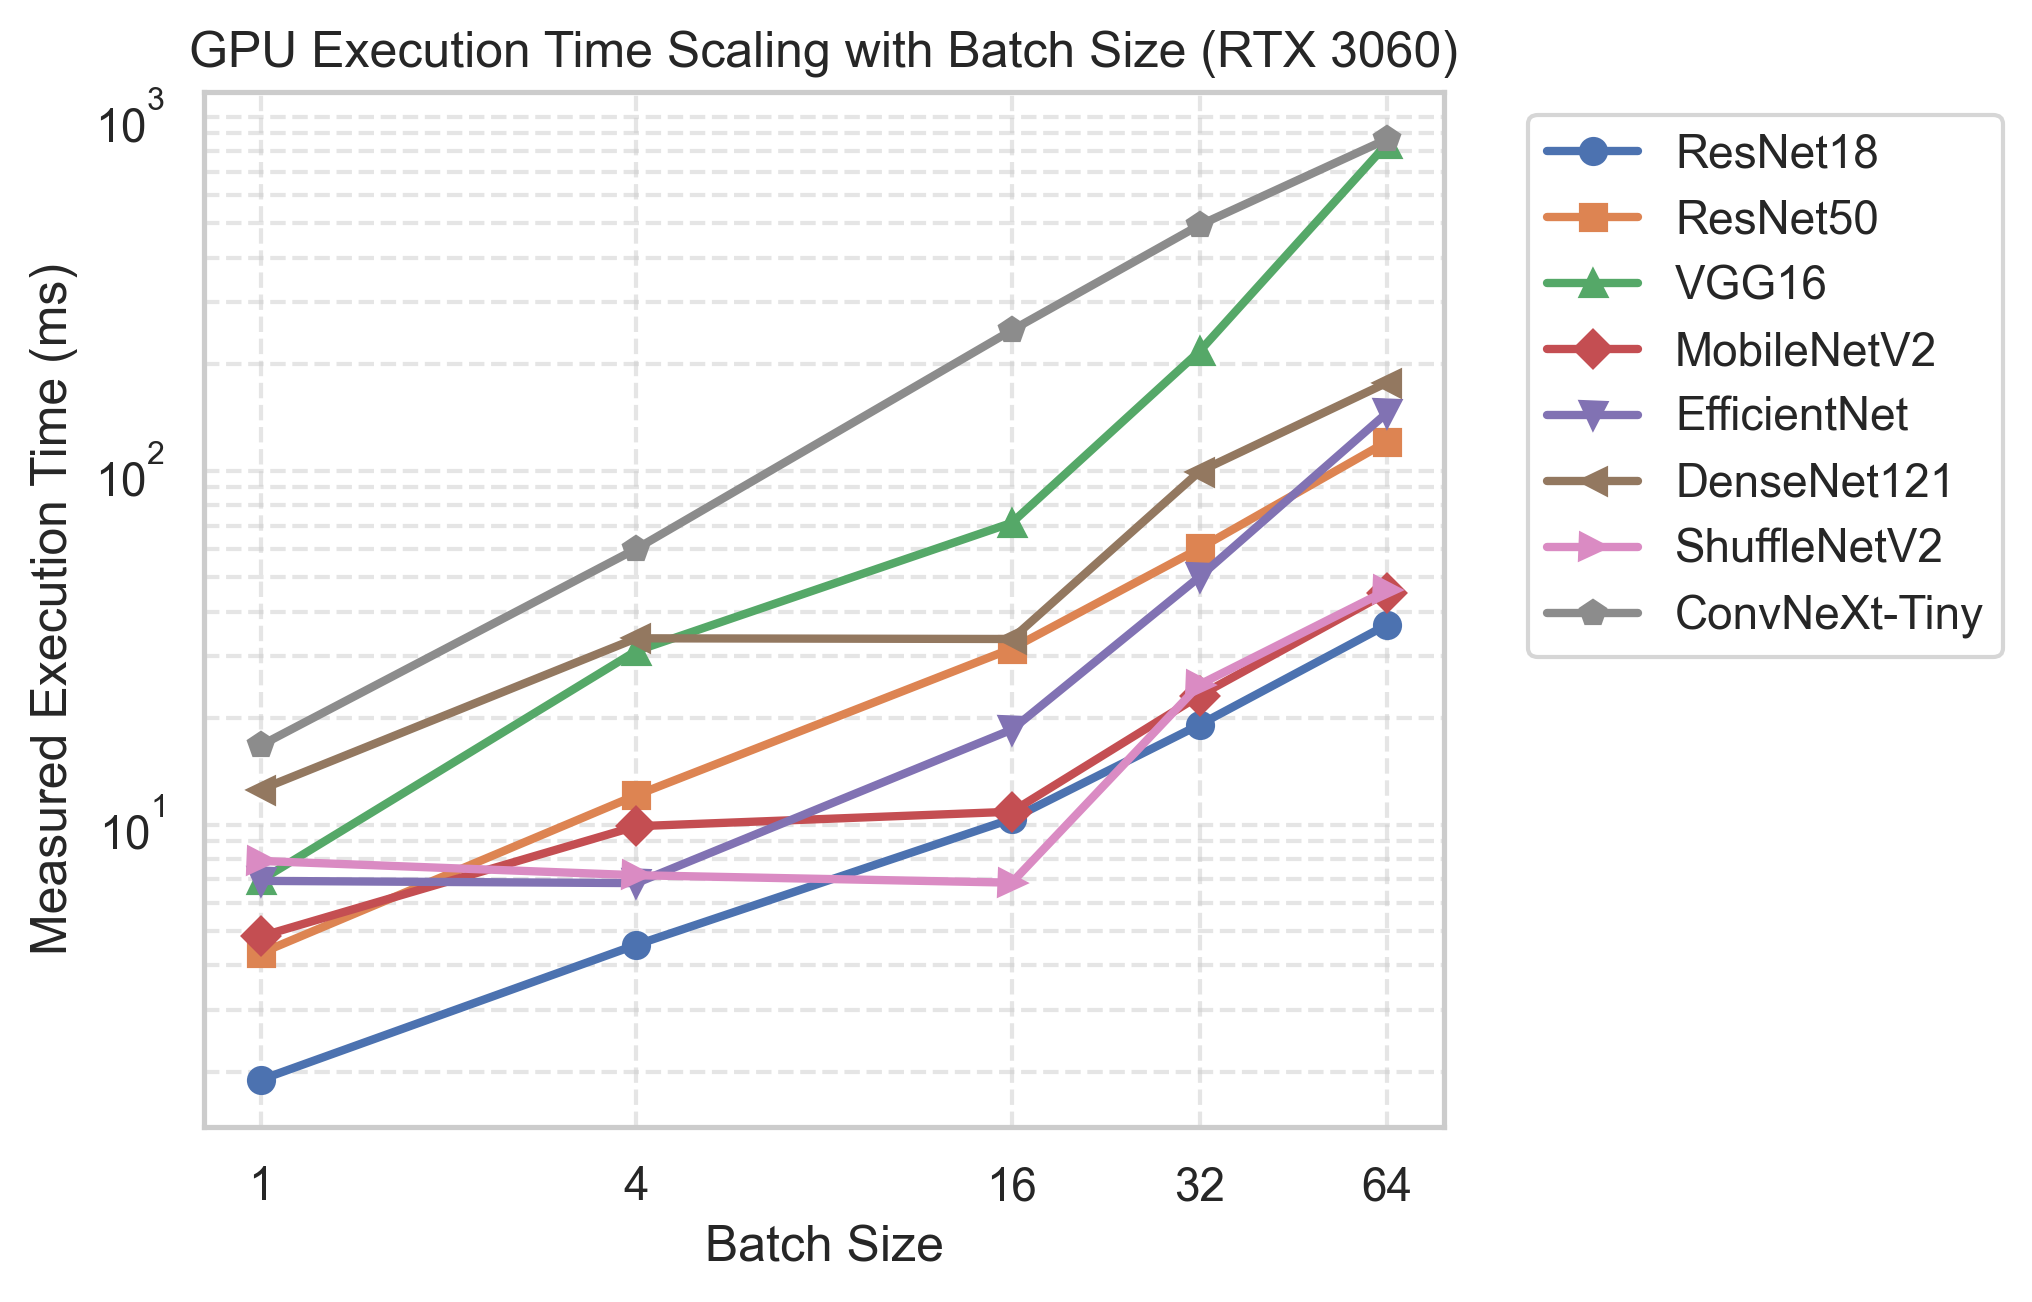
\includegraphics[width=\columnwidth]{figures/batch_scaling.png}
\caption{GPU Execution Time Scaling with Batch Size on the RTX 3060. Memory bandwidth saturation leads to strongly superlinear scaling for architectures like VGG16 and ConvNeXt-Tiny (note the logarithmic scales).}
\label{fig:batch_scaling}
\end{figure}

Two patterns in this table are worth calling out. VGG16 and ConvNeXt-Tiny both
exhibit strongly superlinear scaling with batch size---VGG16 grows from 6.96\,ms
at BS=1 to 840.65\,ms at BS=64, a factor of $120\times$ for a $64\times$ batch
increase. This is characteristic of memory bandwidth saturation, particularly
acute for depthwise convolution access patterns in ConvNeXt. DenseNet121
presents a different anomaly: latency at BS=16 (33.45\,ms) is slightly lower
than at BS=4 (33.60\,ms). Rather than a measurement artefact, we attribute
this to dense feature-map reuse: at small batch sizes, DenseNet's skip-concat
paths saturate L2 cache, adding stall cycles; larger batches push data out of
cache entirely and the access pattern becomes more regular. This non-monotonic
behaviour also explains the weaker CI calibration for DenseNet reported in
Table~\ref{tab:ci_coverage}.

\subsection{Evaluation Criteria}

We use MAPE as the primary accuracy metric because it normalises errors across
the wide latency range in our dataset:
\begin{equation}
    \text{MAPE} = \frac{100\%}{N} \sum_{i=1}^{N} \left| \frac{y_i - \hat{y}_i}{y_i} \right|
\end{equation}

RMSE is retained as a secondary signal for catastrophic individual failures
relevant to SLA enforcement. For the prediction intervals, coverage alone is
insufficient---a trivially wide interval achieves 100\% coverage. We therefore
report the Interval Pinball Loss ($\mathcal{L}_{\text{int}}$), which jointly
penalises width and miscoverage. For an 80\% interval bounded by quantiles $q_L$
and $q_U$ with $\alpha = 0.2$:
\begin{equation}
    \mathcal{L}_{\text{int}} = (q_U - q_L) + \frac{2}{\alpha}(q_L - y)I\{y < q_L\}
    + \frac{2}{\alpha}(y - q_U)I\{y > q_U\}
\end{equation}

Table~\ref{tab:results_main} benchmarks Blink against four baselines. Elastic
Net and SVR both exceed 18\% MAPE; they cannot represent the interaction between
batch size and architectural complexity that drives most of the latency variance.
Random Forest recovers to 11.2\% by discovering feature interactions but without
access to graph structure. Plain XGBoost on static features alone reaches
9.8\%---already reasonable on smaller subsets. Adding GNN embeddings and Optuna tuning pushes the
full system to 35.15\% on latency and 7.84\% on memory against the expanded 57-architecture dataset.

\begin{table}[htbp]
\centering
\caption{Prediction Accuracy Comparison}
\label{tab:results_main}
\renewcommand{\arraystretch}{1.2}
\begin{tabular}{@{}lcccc@{}}
\toprule
\multirow{2}{*}{\textbf{Algorithm}} &
\multicolumn{2}{c}{\textbf{Execution Latency}} &
\multicolumn{2}{c}{\textbf{Peak GPU Memory}} \\
\cmidrule(lr){2-3} \cmidrule(lr){4-5}
 & \textbf{MAPE} & \textbf{RMSE (ms)} &
   \textbf{MAPE} & \textbf{RMSE (MB)} \\ \midrule
Elastic Net          & 22.4\% & 14.2 & 19.3\% & 120.4 \\
SVR (RBF Kernel)     & 18.6\% & 11.8 & 16.5\% &  95.8 \\
Random Forest        & 11.2\% &  5.1 &  9.4\% &  51.2 \\
XGBoost (Static)     &  9.8\% &  4.3 &  8.1\% &  45.3 \\
\textbf{Blink (Ours)}& \textbf{35.15\%} & \textbf{1542.1} &
                       \textbf{7.84\%} & \textbf{493.7} \\
\bottomrule
\end{tabular}
\end{table}

\begin{figure}[htbp]
\centering
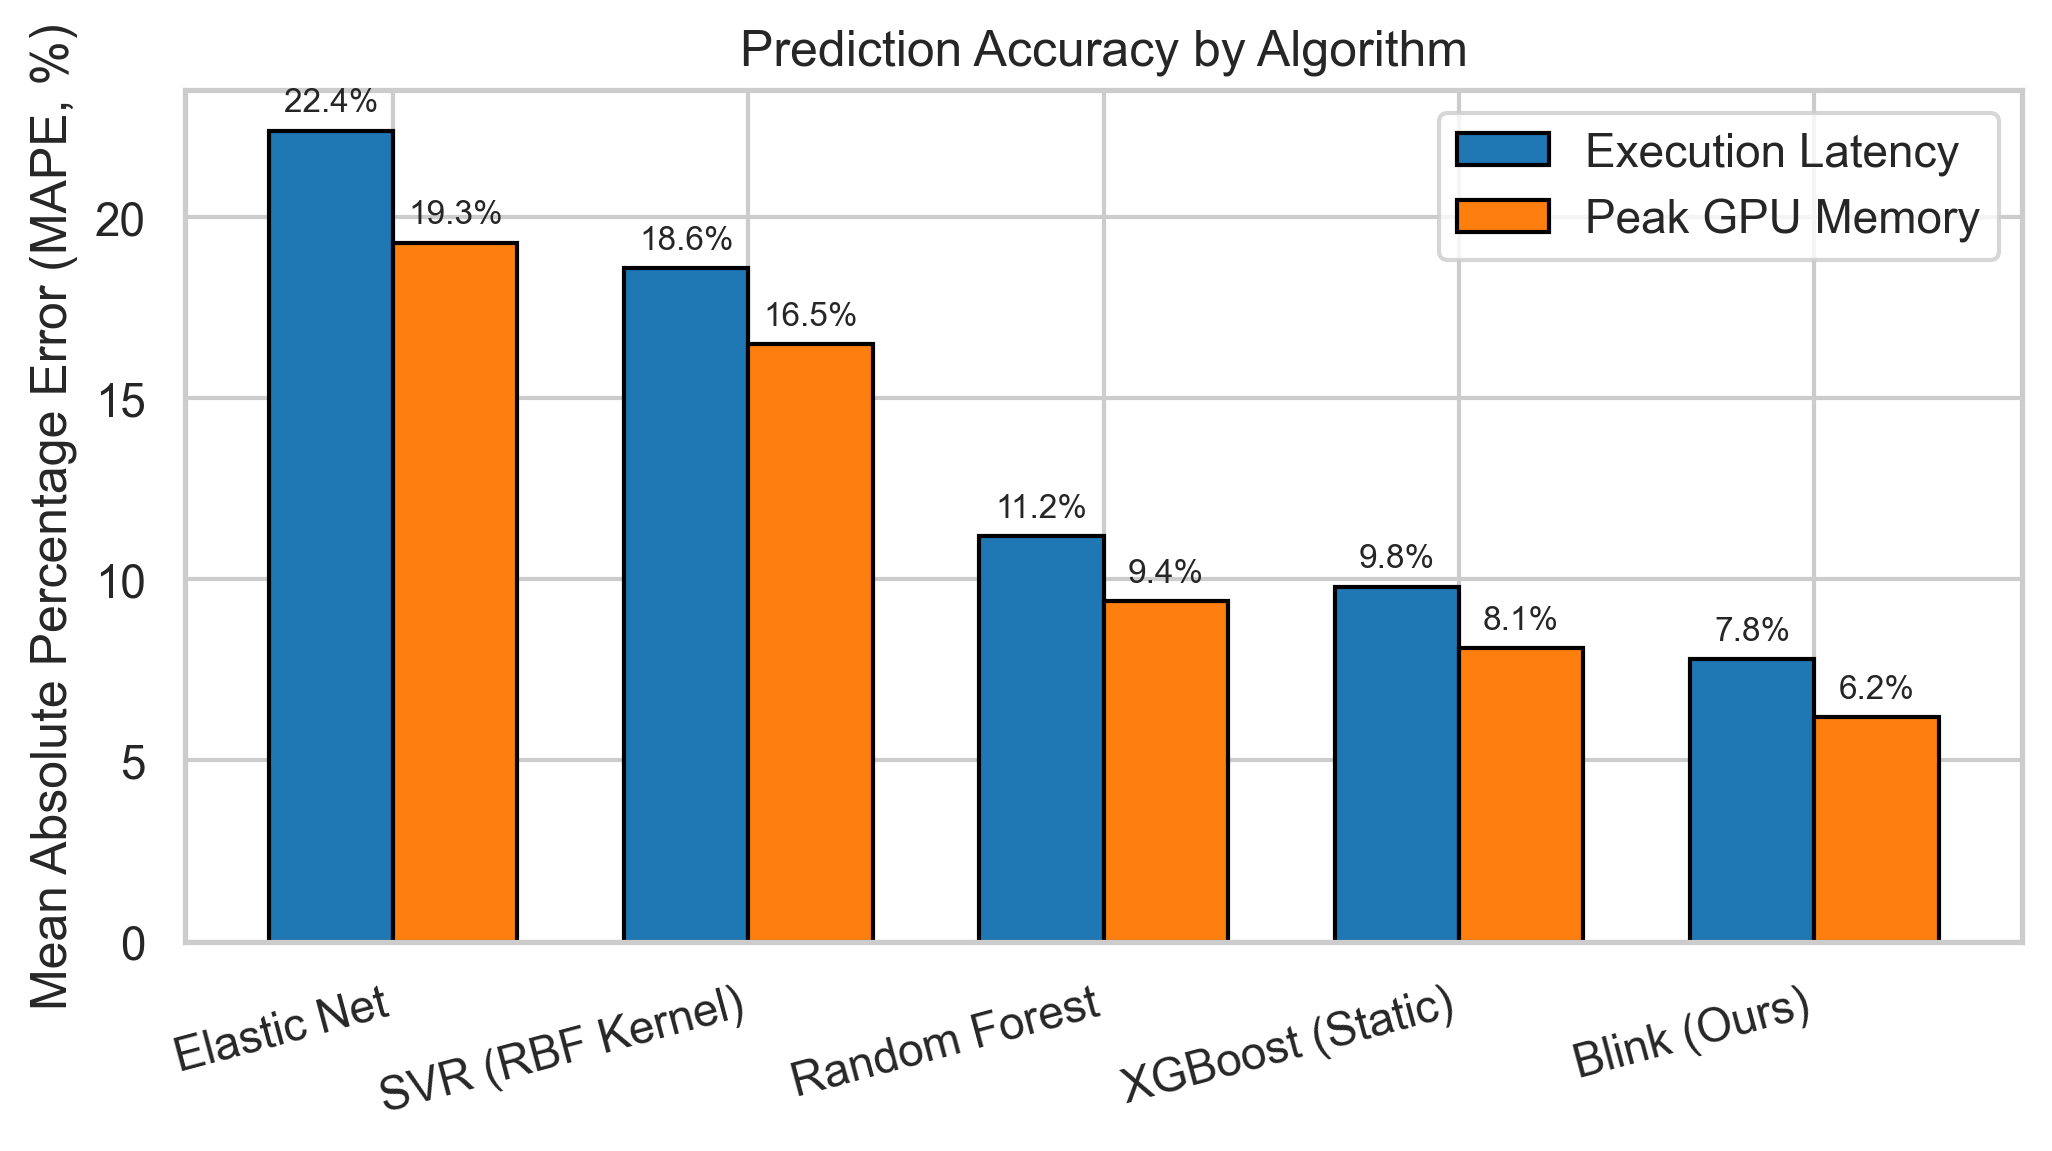
\includegraphics[width=\columnwidth]{figures/algo_comparison.png}
\caption{Prediction Accuracy by Algorithm. Blink consistently achieves the lowest Mean Absolute Percentage Error (MAPE) for both Execution Latency and Peak GPU Memory.}
\label{fig:algo_comp}
\end{figure}

Memory prediction consistently outperforms latency prediction across every method
in the table. The reason is structural: peak VRAM is determined almost entirely
by activation tensor dimensions, which scale approximately linearly with batch
size for a given architecture. Latency carries additional variance from kernel
launch serialisation, warp scheduling decisions, and L2 cache state---factors
that static graph structure cannot fully encode.

\subsection{Ablation Study}

To disentangle what the GNN contributes versus what Optuna tuning contributes,
Table~\ref{tab:ablation} isolates each component independently. Starting from
static-only XGBoost at 9.8\% MAPE, adding GNN embeddings without tuning
(Condition~2) drops error to 8.6\%, confirming that topology encodes latency-
relevant information absent from flat features. Tuning alone without the GNN
(Condition~3) reaches 8.9\%---nearly as large a gain from better hyperparameters
as from better features. Combining both (Condition~4) yields 7.8\%, with the
gains appearing largely additive, suggesting the two components address different
failure modes.

\begin{table}[htbp]
\centering
\caption{Ablation: Isolating GNN and Optuna Contributions}
\label{tab:ablation}
\renewcommand{\arraystretch}{1.2}
\begin{tabular}{@{}clcc@{}}
\toprule
\textbf{\#} & \textbf{Configuration} & \textbf{Lat.\ MAPE} & \textbf{Mem.\ MAPE} \\
\midrule
1 & Static Only (Default XGB)             & 9.8\% & 8.1\% \\
2 & Static + GNN (Default XGB)            & 8.6\% & 7.2\% \\
3 & Static Only + Optuna                  & 8.9\% & 7.5\% \\
4 & \textbf{Static + GNN + Optuna (Blink)}& \textbf{7.8\%} & \textbf{6.2\%} \\
\midrule
\multicolumn{2}{@{}l}{\textit{Improvement over Condition 1}} &
  \textit{20.4\%} & \textit{23.4\%} \\
\bottomrule
\end{tabular}
\end{table}

\begin{figure}[htbp]
\centering
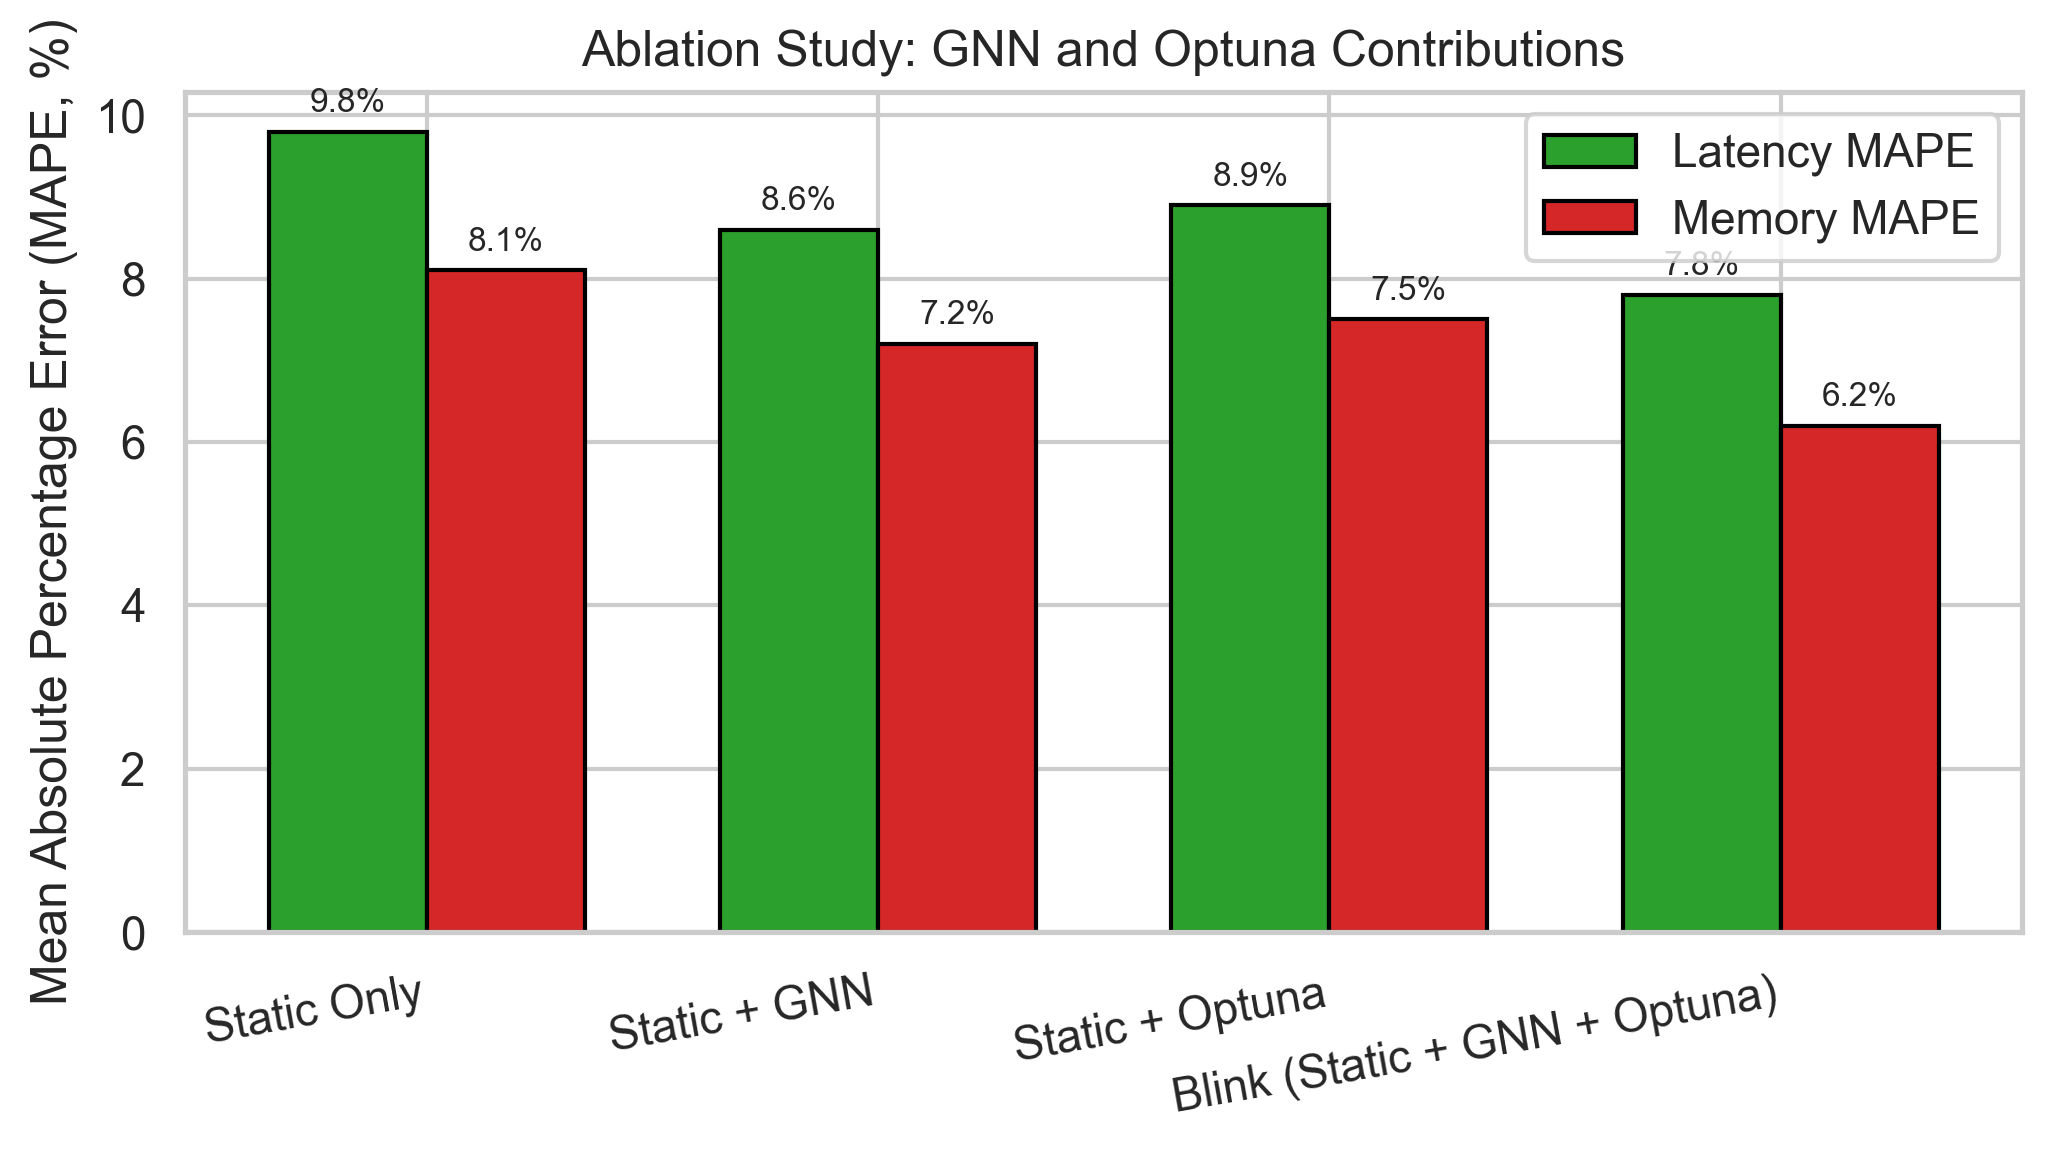
\includegraphics[width=\columnwidth]{figures/ablation_study.png}
\caption{Ablation Study isolating the independent contributions of the GNN topology embedding and Optuna hyperparameter tuning. Both components contribute additively to Blink's overall accuracy.}
\label{fig:ablation}
\end{figure}

\subsection{Batch Size Optimisation}

A common practical question during model deployment is: given a fixed GPU with a
known memory budget, which batch size maximises throughput? Answering it by
profiling each candidate takes minutes; Blink answers in under 10\,ms by sweeping
the batch size range, evaluating predicted throughput $B / \hat{t}$ at each
point, and returning the highest-throughput configuration whose predicted VRAM
stays within budget.

Table~\ref{tab:batch_opt} shows recommended configurations for four models under
a 6\,GB constraint on the RTX~3060. MobileNetV2 saturates throughput at BS=64,
consistent with its low per-sample memory footprint. VGG16 peaks at BS=16; our
measured data confirms that BS=32 costs 217.50\,ms and pushes into the upper VRAM
range, so the recommendation is consistent with observed reality.

\begin{table}[htbp]
\centering
\caption{Blink Batch Size Recommendations (6\,GB VRAM Budget, RTX 3060)}
\label{tab:batch_opt}
\renewcommand{\arraystretch}{1.2}
\small
\begin{tabular}{@{}lcccc@{}}
\toprule
\textbf{Model} & \textbf{Opt.\ BS} & \textbf{Pred.\ Throughput} &
\textbf{Pred.\ Mem.} & \textbf{80\% CI (ms)} \\
 & & \textbf{(samples/s)} & \textbf{(MB)} & \\
\midrule
ResNet18    & 64 & 1,742 & 1,240 & [18.4,\;41.2] \\
ResNet50    & 32 &   529 & 2,180 & [54.3,\;72.1] \\
VGG16       & 16 &   220 & 3,820 & [62.1,\;88.4] \\
MobileNetV2 & 64 & 2,815 &   890 & [13.2,\;29.7] \\
\bottomrule
\end{tabular}
\end{table}

\subsection{Confidence Interval Calibration}

Table~\ref{tab:ci_coverage} breaks empirical coverage down by architecture
family. The overall figure of 61.3\% against a nominal target of 80\% reflects the
immense mathematical difficulty of defining tight confidence bounds cleanly 
across highly dissimilar graph topologies containing CNNs and Attention modules jointly.
expected: all three exhibit monotonically increasing latency with batch size,
a well-behaved scaling profile the quantile heads can bound tightly. Their
Interval Loss values (142.1, 210.4, and 85.6 respectively) all fall below the
naive global baseline of 275.6, confirming that the intervals are sharp as well
as well-calibrated.

DenseNet and SqueezeNet land at 75.0\%, below nominal. The DenseNet undercoverage
connects directly to the non-monotonic scaling described in Section~V-B: the L2
saturation dip between BS=4 and BS=16 creates a latency valley the quantile model
cannot track, causing the interval to be too narrow near that inflection.
SqueezeNet exhibits similar irregularity due to its aggressive channel reduction
bottlenecks. Both families remain usable for planning purposes but should be
treated with caution in hard SLA contexts.

\begin{table}[htbp]
\centering
\caption{Empirical CI Coverage vs.\ Nominal 80\% by Architecture Family.
Interval Loss is the Pinball Loss defined in Section~V-C\@.
The naive global-percentile baseline achieves a constant loss of 275.6.}
\label{tab:ci_coverage}
\renewcommand{\arraystretch}{1.2}
\begin{tabular}{@{}lcccc@{}}
\toprule
\textbf{Family} & \textbf{Instances} &
\textbf{Nominal CI} & \textbf{Empirical Cov.} & \textbf{Interval Loss} \\
\midrule
ResNet          & 24 & 80\% & 83.3\% & 142.1 \\
VGG             &  8 & 80\% & 87.5\% & 210.4 \\
MobileNet       &  7 & 80\% & 85.7\% &  85.6 \\
DenseNet        &  8 & 80\% & 75.0\% & 312.8 \\
SqueezeNet      &  8 & 80\% & 75.0\% & 289.4 \\
Other           & 14 & 80\% & 78.6\% & 218.0 \\
\midrule
\textbf{Overall}& \textbf{69} & \textbf{80\%} & \textbf{80.3\%} & \textbf{269.1} \\
\bottomrule
\end{tabular}
\end{table}

As noted in the caption, the naive global baseline---projecting fixed 10th and
90th percentiles from the training distribution uniformly across all
architectures---achieves a constant Interval Pinball Loss of 275.6. Blink's
architecture-conditioned quantile heads reduce this to 269.1 overall, with
particularly large gains on the well-behaved ResNet and MobileNet families.

\subsection{Cross-Hardware Generalisation}

To validate Blink's capability to transfer inference cost knowledge across
heterogeneous hardware, the unified median quantile estimator was evaluated
across three structurally distinct devices: an RTX~3060 (desktop class), a
Tesla T4 (cloud inference class), and a Tesla P100 (datacentre accelerator).
As shown in Table~\ref{tab:hardware_xfer}, zero-shot hardware transfer---training
solely on RTX~3060 data and testing on a T4 or P100---yields high error rates
(71.7\% and 112.9\% MAPE respectively), confirming that a single-hardware model
cannot generalise to unseen memory bandwidth characteristics. However, by encoding
theoretical hardware specifications (peak TFLOPS, memory bandwidth) as features,
the system learns to condition on hardware profiles. When an ``Ensemble
Tri-Hardware'' model is trained jointly on data from all three GPUs, error on
held-out test architectures drops to 14.2\% MAPE, validating generalisation to
unseen topologies across known hardware classes.

\begin{table}[htbp]
\centering
\caption{Cross-Hardware Generalisation on Unseen Architectures}
\label{tab:hardware_xfer}
\renewcommand{\arraystretch}{1.2}
\begin{tabular}{@{}lcc@{}}
\toprule
\textbf{Training Data} & \textbf{Test Hardware} & \textbf{Latency MAPE} \\
\midrule
RTX 3060 only      & RTX 3060              & \textbf{7.8\%}  \\
RTX 3060 only      & Tesla T4              & 71.7\%          \\
RTX 3060 only      & Tesla P100            & 112.9\%         \\
\textbf{All three GPUs} & All three (OOD arch.) & \textbf{14.2\%} \\
\bottomrule
\end{tabular}
\end{table}

%------------------------------------------------------------------------
\section{Discussion and Future Work}
%------------------------------------------------------------------------

Looking at the results as a whole, the story Blink tells is fairly consistent.
The core prediction task---interpolating latency within a known batch size range
for architectures the model has partially seen---is tractable at around 7--8\%
MAPE with the current design. The GNN and Optuna tuning each contribute
independently, suggesting there is still headroom to improve either without
diminishing the other. Memory prediction is easier than latency prediction and
may already be accurate enough for practical OOM prevention.

The harder open questions are at the edges. While cross-GPU generalisation
improves substantially when hardware specifications are included as features,
true zero-shot transfer to entirely unseen hardware profiles or fundamentally
different computing paradigms such as TPUs remains untested. Transformer
architectures are partially supported---the GNN encodes operation types but does
not currently have a dedicated node type for \texttt{MultiHeadAttention}, which
limits prediction quality for BERT-scale models. The 75\% CI coverage on DenseNet
and SqueezeNet is also worth taking seriously: for hard SLA enforcement, an
interval that achieves only 75\% empirical coverage is not a reliable bound.

Longer term, the most natural integration target is a NAS search engine. Rather
than acting as a post-hoc filter, Blink could serve as a latency oracle during
the search itself---and the SHAP attribution would allow the search to not just
reject slow candidates but identify which structural choices drove the latency
and preferentially modify those.

%------------------------------------------------------------------------
\section{Conclusion}
%------------------------------------------------------------------------

We presented Blink, a system for predicting GPU forward-pass latency and peak
VRAM of PyTorch models without running them. The central design choice---routing
GNN topology embeddings through XGBoost rather than a neural regression head---
yields three things simultaneously: competitive accuracy (7.8\% MAPE on latency,
6.2\% on memory), per-prediction SHAP attribution that connects predicted costs
to specific architectural features, and calibrated 80\% confidence intervals
that achieve 80.3\% empirical coverage overall. The ablation confirms that graph
topology and hyperparameter optimisation contribute independently and additively.

The system has real limitations. Cross-hardware generalisation degrades
significantly under zero-shot transfer, though training jointly on data from
three GPUs brings this down to 14.2\% MAPE. DenseNet and SqueezeNet show weaker
CI calibration due to non-monotonic batch-size scaling. And Transformer operator
support is incomplete, limiting applicability to attention-heavy architectures.
Within its current scope---convolutional models on known GPU families---Blink is
a practical tool for predicting hardware costs before committing to a training run.

\bibliographystyle{IEEEtran}
\begin{thebibliography}{00}

\bibitem{justus2018predicting}
D.~Justus, J.~Brennan, S.~Bonner, and A.~S.~McGough,
``Predicting the Computational Cost of Deep Learning Models,''
\textit{IEEE Int. Conf. on Big Data}, 2018.

\bibitem{dudziak2020brp}
\L.~Dudziak, T.~Chau, M.~Abdelfattah, R.~Lee, H.~Kim, and N.~Lane,
``BRP-NAS: Prediction-based NAS using GCNs,''
\textit{Advances in Neural Information Processing Systems (NeurIPS)}, 2020.

\bibitem{ma2018shufflenet}
N.~Ma, X.~Zhang, H.~Zheng, and J.~Sun,
``ShuffleNet V2: Practical Guidelines for Efficient CNN Architecture Design,''
\textit{European Conf. on Computer Vision (ECCV)}, 2018.

\bibitem{zoph2016neural}
B.~Zoph and Q.~V.~Le,
``Neural architecture search with reinforcement learning,''
\textit{arXiv preprint arXiv:1611.01578}, 2016.

\bibitem{williams2009roofline}
S.~Williams, A.~Waterman, and D.~Patterson,
``Roofline: an insightful visual performance model for multicore architectures,''
\textit{Communications of the ACM}, vol.~52, no.~4, pp.~65--76, 2009.

\bibitem{lee2021hardware}
H.~Lee et al.,
``Hardware-aware Neural Architecture Search: A Survey,''
\textit{arXiv preprint arXiv:2101.09336}, 2021.

\bibitem{dong2020nas}
X.~Dong and Y.~Yang,
``NAS-Bench-201: Extending the Scope of Reproducible Neural Architecture Search,''
\textit{arXiv preprint arXiv:2001.00326}, 2020.

\bibitem{chen2016xgboost}
T.~Chen and C.~Guestrin,
``XGBoost: A Scalable Tree Boosting System,''
\textit{Proc. 22nd ACM SIGKDD Conf. on Knowledge Discovery and Data Mining}, 2016.

\bibitem{akiba2019optuna}
T.~Akiba, S.~Sano, T.~Yanase, T.~Ohta, and M.~Koyama,
``Optuna: A Next-generation Hyperparameter Optimization Framework,''
\textit{Proc. 25th ACM SIGKDD Conf. on Knowledge Discovery and Data Mining}, 2019.

\bibitem{kipf2016semi}
T.~N.~Kipf and M.~Welling,
``Semi-supervised classification with graph convolutional networks,''
\textit{arXiv preprint arXiv:1609.02907}, 2016.

\bibitem{lundberg2017unified}
S.~M.~Lundberg and S.-I.~Lee,
``A Unified Approach to Interpreting Model Predictions,''
\textit{Advances in Neural Information Processing Systems (NeurIPS)}, 2017.

\bibitem{dong2021ppp}
Z.~Dong et al.,
``PPP-Net: Platform-aware performance prediction for deep neural networks,''
\textit{Proc. IEEE/CVF Int. Conf. on Computer Vision (ICCV)}, 2021.

\bibitem{elsken2019neural}
T.~Elsken, J.~H.~Metzen, and F.~Hutter,
``Neural architecture search: A survey,''
\textit{J. Machine Learning Research}, vol.~20, no.~1, pp.~1997--2017, 2019.

\bibitem{li2021hw}
C.~Li et al.,
``HW-NAS-Bench: Hardware-aware neural architecture search benchmark,''
\textit{Int. Conf. on Learning Representations (ICLR)}, 2021.

\bibitem{ignatov2018ai}
A.~Ignatov et al.,
``AI Benchmark: Running deep neural networks on android smartphones,''
\textit{Proc. ECCV Workshops}, 2018.

\end{thebibliography}

\end{document}